\documentclass[sigconf,anonymous,review]{acmart}

% Anonymous review version; publication metadata is assigned after acceptance.
\setcopyright{none}
\settopmatter{printacmref=true}
\acmDOI{}
\acmISBN{}
\acmConference[WWW '27]{The ACM Web Conference 2027}{May 10--14, 2027}{Dublin, Ireland}
\acmYear{2027}
\copyrightyear{2027}

\usepackage{graphicx}
\usepackage{amsmath}
\usepackage{textcomp}
\usepackage{xcolor}
\usepackage{tabularx}
\usepackage{booktabs}
\usepackage{algorithm}
\usepackage{algpseudocode}
\usepackage{url}
\usepackage{xspace}
\usepackage{cleveref}
\crefname{section}{\S}{\S\S}
\Crefname{section}{\S}{\S\S}
\newcommand{\sys}{\mbox{WebRouteMap}\xspace}

\begin{document}
\title[WebRouteMap: Which Networks Carry Your Web Traffic?]{WebRouteMap: Which Networks Carry Your Web Traffic?}
\author{Anonymous Author(s)}

\begin{abstract}
Web access depends on intermediary networks that are difficult for users and
content providers to see. A path view could help users inspect transit
dependencies and providers compare access to serving locations, but direct
measurements require vantage points in the relevant user networks. We present
\sys, a tool that estimates the autonomous-system (AS) paths behind Web access
without measurements from every target user network. Given a user network and
a selected website endpoint, it combines public routing observations with
interconnection metadata to rank possible exits, extend branches with sparse
continuations, and score complete paths using destination-specific propagation
evidence. A shared selected path library supports training and candidate
generation; an existing ranker then answers individual path queries. We evaluate a controlled BGP
source-withholding experiment, whose destinations represent potential
Web-service locations, and independent traceroutes to domain-derived endpoints.
The three-snapshot BGP benchmark obtains approximately 80\% AS-set Jaccard,
using ten source ASes per date. The single-source Web experiment obtains 69.96\% over 1,890 pairs,
compared with 69.19\% for KnownPath. The evaluations quantify network-path agreement for Web access.
\end{abstract}

\ccsdesc[500]{Networks~Network measurement}
\keywords{Web access, network-path visibility, public routing evidence, AS-level routing}
\maketitle

\section{Introduction}
\label{sec:introduction}

\emph{Which networks carry a user's traffic when visiting websites?} Domain
names identify services but reveal little about the intermediary networks
connecting users to their serving endpoints. A user reading news, shopping,
and streaming video may depend on a common transit network despite visiting
different services (Figure~\ref{fig:motivation}). At the autonomous-system
(AS) level, visibility into these paths could help users inspect their
exposure to intermediary networks and help content providers compare how
user networks reach candidate serving locations. This view complements
studies of hosting, DNS, and certificate
dependencies~\cite{kashaf2020dependencies,habib2025dependence} by examining
the networks connecting users to Web services.

\begin{figure}[t]
\centering
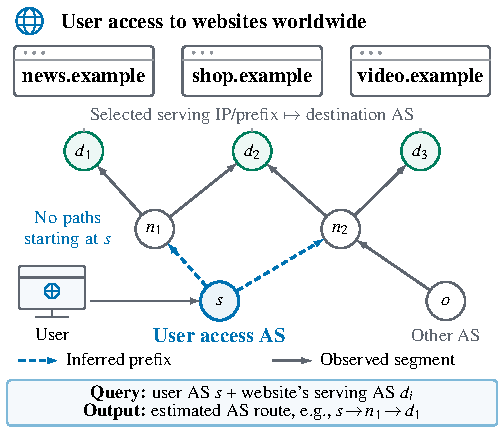
\includegraphics[width=\columnwidth]{figures/fig1_scenario.pdf}
\caption{Network paths behind Web access. For each externally supplied
serving AS $d_i$, \sys joins an estimated prefix with an observed segment to
estimate the user's route. Dashed and solid arrows distinguish the two
sources of evidence. The diagram shows AS connectivity, not geography.}
\Description{A user in access AS s visits news, shopping, and video services.
Dashed prefixes connect s to n1 and n2; solid publicly observed segments
continue to serving ASes. Both branches can reach the shopping service.
Another source AS supplies indirect observations.}
\label{fig:motivation}
\end{figure}

Obtaining this visibility across user networks is difficult. Traceroute
observes paths from deployed probes, so coverage depends on suitable
vantage points~\cite{tracerouteJacobson,RIPEAtlas}. Public BGP collectors add
routing observations from participating networks, but their coverage is
incomplete~\cite{RouteViews,RIPERIS,huffaker2023importance}. Path inference
extends these observations. Graph-based methods can generate routes without
source-originated measurements, yet simplified policy rules cannot fully
capture source-specific routing behavior~\cite{qiu2005path,11044440}.
Stitching methods reuse observed segments, but composition alone cannot
construct a route when suitable source-connected segments are
absent~\cite{probinfer}. Hybrid methods improve coverage, while uneven
observations remain a challenge across source networks~\cite{11044440}.

The shortage of source observations creates a cold-start problem for
learning-based inference. For example, GMPI trains a source-specific model
using observed paths rooted at the source AS~\cite{li2023realizing}; few or no such paths leave
insufficient supervision for learning its routing
behavior~\cite{li2024internet}. PA-GMPI introduces adaptive training and
warm-start mechanisms~\cite{li2024realizing}.
We ask: \emph{Can we make the network paths behind Web access visible to users
and content providers, without requiring path measurements from every user
network?} To address this cold start, we use public interconnection
information to connect the source to route segments observed from other
networks. This path augmentation provides plausible source-rooted training
paths for learning routes from user networks to website endpoints.

Constructing these training paths presents three challenges.
\textbf{First, how should likely forwarding branches be identified and
explored?} Well-observed neighbors can supply many reusable paths, whereas
poorly observed neighbors require further exploration. When a source has
few neighbors, important routing choices may lie beyond its first hop.
Neighbor selection and recursive exploration must therefore determine
which branches to follow and where usable observations become available.
\textbf{Second, how should paths be generated and selected?} Graph search
or stitching can produce paths the source would not use. Construction must
be coupled with reliability assessment and selection that preserves
important neighbors.
\textbf{Third, how can public evidence inform these decisions without AS
configurations or direct source measurements?} BGP paths, AS relationships,
and interconnection metadata describe different aspects of routing and have
uneven coverage. Their information requires representations of ASes,
forwarding transitions, and complete paths that account for source and
destination context while preserving missing or uncertain evidence.

We present \textbf{\sys}, a Web-path visibility framework that estimates
routes from user networks to selected website endpoints using public routing
observations and interconnection metadata.

\textbf{To address the first challenge,} we combine learned neighbor
ranking with evidence-guided recursive exploration. A source-level ranker
prioritizes neighbors through which the source is likely to forward
traffic. For each selected neighbor, we count observed continuations that
can form structurally admissible training paths. Sufficient evidence
allows direct reuse; otherwise, a local ranker identifies supported next
hops for bounded prefix expansion. We retain prefixes with usable
continuations alongside their extensions, preserving sparse evidence
while exploring routing choices beyond the source's immediate neighbors.

\textbf{To address the second challenge,} we combine observed-path
stitching with learned complete-path scoring and neighbor-aware selection.
Observed BGP paths encode routing choices made by real networks, so
reusing intact segments reduces how much of a training path must be
inferred. We connect the source to segments rooted at selected neighbors
or recursively reached ASes, preserving their direction and order. A
learned scorer estimates observation support for the complete candidate.
Selection reserves available samples through important neighbors before
filling the remaining budget with high-scoring alternatives, keeping
important forwarding branches represented in the training library.

\textbf{To address the third challenge,} we build a multilevel
representation of public routing and interconnection evidence. AS
features describe network roles, connectivity, and PeeringDB co-location;
transition features capture directed commercial relationships and local
routing support; path features summarize prefix reliability and observed
segment support. Destination-specific evidence measures agreement among
other source networks under comparable incoming commercial roles.
Per-source normalization and equal source weighting limit dominance by
prolific observers, while explicit missingness and conflict indicators
preserve uncertainty. These representations support neighbor ranking,
recursive exploration, and complete-path assessment without private AS
configurations.

Our implementation uses GMPI for path inference, with the selected library
supplying training paths and evidence for candidate generation in
user-to-website queries such as those in Figure~\ref{fig:motivation}.

We make three contributions:
\begin{itemize}
\item We present \sys, a framework that estimates AS-level paths from user
networks to selected website endpoints without requiring path measurements
from the target user network.
\item We develop an evidence-guided path-augmentation method for ASes
without source-originated measurements. Using multilevel public evidence,
it combines learned neighbor selection, recursive exploration, and
observed-segment stitching with complete-path scoring and sample safeguards
for important neighbors.
\item We validate \sys in two complementary settings: a controlled BGP
source-withholding benchmark across three snapshots and an independent
traceroute experiment toward domain-derived endpoints. Stage-wise
evaluation measures neighbor coverage and augmented-path observation
support, alongside final AS-set Jaccard.
\end{itemize}

\section{Background and Related Work}
\label{sec:background}

\subsection{Web Access and Interdomain Routes}

A user's route to a website depends on its access network and serving
endpoint. DNS steering can select different server addresses, while anycast
can reach different serving instances at the same
address~\cite{schomp2020akamai,koch2021anycast,kumar2026steering}.
Mapping the endpoint prefix to an AS defines an interdomain query, although
prefixes within that AS may follow different routes. This view complements
Web-dependency research~\cite{kashaf2020dependencies,habib2025dependence}
by examining the networks connecting users to selected endpoints.

BGP distinguishes learning a route from a neighbor, selecting it under
local policy, and exporting it to other neighbors~\cite{rfc4271}.
Route Views and RIPE RIS expose paths advertised by participating
networks~\cite{RouteViews,RIPERIS}. CAIDA relationships, ASRank, and
PeeringDB add commercial roles, network attributes, and shared IXP or
facility presence~\cite{CAIDA,caidaASrank,PeeringDB}. These sources
constrain possible routes, but do not disclose all private preferences.
Co-location does not establish a connection, and valley-free compatibility
does not establish that a network uses a particular
route~\cite{gao2001inferring}.

\subsection{Direct Path Measurement}

Traceroute varies the IP time-to-live to collect replies from forwarding
hops~\cite{tracerouteJacobson}. Its output describes an observation from
a particular source toward a target at the measurement time. Classic
traceroute can combine replies from different paths under load balancing;
Paris traceroute controls flow identifiers to reduce per-flow
artifacts~\cite{ParisTraceroute}. It does not eliminate every form of
load balancing or measurement uncertainty. Scamper supports parallel,
rate-controlled probing, while RIPE Atlas provides distributed probes for
user-defined measurements~\cite{scamper2010,RIPEAtlas}.

These tools support large-scale measurement, but directly observing paths
from a user AS requires an available vantage point there~\cite{RIPEAtlas}.
Repeated probing consumes measurement resources. Unresponsive hops and filtering can
leave gaps~\cite{RIPEAtlasResultFormat}, and converting IP replies into AS
sequences introduces mapping uncertainty~\cite{mao2003AStraceroute}. BGP paths
provide control-plane evidence and need not match a traceroute's
data-plane sequence. Direct measurement and inference are complementary:
measurements supply observations, while inference estimates paths from
user networks without a suitable source probe.

\subsection{AS Path Inference}

AS-path inference estimates unmeasured routes from available
evidence~\cite{li2024internet}.
\textbf{KnownPath} exploits AS paths already present in BGP tables to infer
routes from a source AS to a destination prefix~\cite{qiu2005path}.
\textbf{ProbInfer} represents observed path segments in a multigraph and
combines segment composition with probability-based candidate evaluation,
using public passive measurement data~\cite{probinfer}.

\textbf{GMPI} combines heuristic candidate-path generation with a neural
evaluation model. It integrates topology and AS attributes with related
observed paths through path representations and dual
attention~\cite{li2023realizing}.
\textbf{PA-GMPI} extends this approach with personalized path generation
and adaptive model training using information specific to individual
ASes. It introduces a graph-kernel-based training warm starter and an AS
representation learner based on observed walks~\cite{li2024realizing}.
These works address candidate generation, evidence integration, and
source-specific inference; we reuse the existing GMPI-based downstream
ranking stage.

\textbf{PathRadar} distinguishes core and shell ASes according to routing
complexity and observation adequacy, combining policy-based and
stitching-based inference. Its progressive learning process propagates and
evaluates candidate routes; it also addresses prefix-specific paths,
multiple paths per AS pair, and selected non-valley-free path
patterns~\cite{11044440}.

Other systems provide complementary perspectives: iPlane composes observed
segments to predict paths and their properties~\cite{madhyastha2006iplane,madhyastha2009iplane};
PredictRoute combines historical data- and control-plane evidence with
probabilistic path prediction~\cite{singh2021predictroute}; and RouteInfer
models diversity and commonality in ISP routing
behavior~\cite{wang2022routeinfer}. Our focus is source-specific evidence
construction for Web-path queries when paths originating from the user
network are unavailable. We combine learned neighbor selection, expansion
of evidence-poor branches, and complete-path support scoring to produce
one selected library for both training and candidate generation. This
construction complements the downstream inference model.

\section{Problem Setting}
\label{sec:problem}

\subsection{Web-Path Queries and Scope}

A query supplies a source AS $s$, destination AS $d$ obtained from a selected
website endpoint, and routing snapshot $t$. The tool returns an ordered
forward AS sequence $\widehat P_{s,d}$ or reports that no usable candidate is
available. The same snapshot allows evidence to be reused across endpoint
queries. This is the tool's output;
constructed paths used to answer the queries are intermediate evidence.

The AS-pair abstraction groups prefixes and endpoints within the same AS.
It estimates interdomain connectivity, not routers, geography, the return
path, or the forwarding path of every Web request. The BGP experiment models
destination ASes as potential Web-service networks; it does not establish
that every such AS hosts a website. The domain-endpoint experiment separately
tests destinations obtained by resolving a popular-domain list.

\subsection{Public Evidence and Reusable Path Segments}

Let $\mathcal P$ be the collected AS paths available at a snapshot, excluding
paths that start at the target source. The source may occur internally in a
path from another network. We build a graph $\mathcal G$ from adjacent ASes
and use archived relationship and network-metadata bundles.
Table~\ref{tab:notation} defines the principal symbols.

\begin{table}[t]
\centering
\caption{Query inputs and intermediate evidence.}
\label{tab:notation}
\footnotesize
\begin{tabularx}{\columnwidth}{@{}lX@{}}
\toprule
Symbol & Meaning\\
\midrule
$s,d$ & User-network and selected endpoint AS\\
$\mathcal P,\mathcal G$ & Public path corpus and its AS graph\\
$\Gamma(u),\rho(u,v)$ & Graph neighbors and directed AS relationship\\
$\mathcal N_s,\mathcal A_{s,n}$ & Admitted first hops and recursive anchors\\
$T_{z,j}(P),F(T)$ & Directed segment rooted at $z$, and its frequency\\
$\mathcal U_s,\mathcal K_s$ & Augmentation shortlist and observed source-rooted suffixes\\
$\mathcal R_s,\pi_s(n)$ & Selected path library and predicted first-hop importance\\
$\mathcal C_{s,d},\widehat P_{s,d}$ & Query candidates and returned route estimate\\
\bottomrule
\end{tabularx}
\end{table}

For $P=(v_0,\ldots,v_\ell)\in\mathcal P$ with $z=v_i$, a reusable segment is
\begin{equation}
T_{z,j}(P)=(v_i,\ldots,v_j),\qquad i<j\leq\ell.
\label{eq:collected_tail}
\end{equation}
Segments in~\eqref{eq:collected_tail} retain their observed direction and
interior AS sequence; their endpoint may be internal to the parent path.
The special case $z=s$ and $j=\ell$ yields a complete source-rooted suffix
when $s$ occurs internally. We denote these original-terminal suffixes by
$\mathcal K_s$. We never reverse an observation to manufacture a forward
route.

\subsection{Training Library and Inference Objective}

We seek a source-specific library $\mathcal R_s$ that supplies training
paths for learning the source's routing behavior without measurements
originating from $s$. The library contains augmented paths and eligible
observed suffixes from $\mathcal K_s$, retaining examples through important
forwarding neighbors. The same library supports model training and local
candidate generation. Given a candidate set $\mathcal C_{s,d}$, the query
objective is to select
\begin{equation}
\widehat P_{s,d}
=\underset{P\in\mathcal C_{s,d}}{\arg\max}\; f_{\theta_s}(P,H_{s,d}),
\label{eq:downstream_inference}
\end{equation}
where $H_{s,d}$ is the available query-specific path history and
$f_{\theta_s}$ is a learned source-specific path score. Library construction
provides reusable supervision; query inference chooses one route for the
requested endpoint. Scores express relative preference among candidates.

\section{WebRouteMap Design}
\label{sec:neighbors}

\subsection{Framework Overview}

\begin{figure*}[t]
\centering
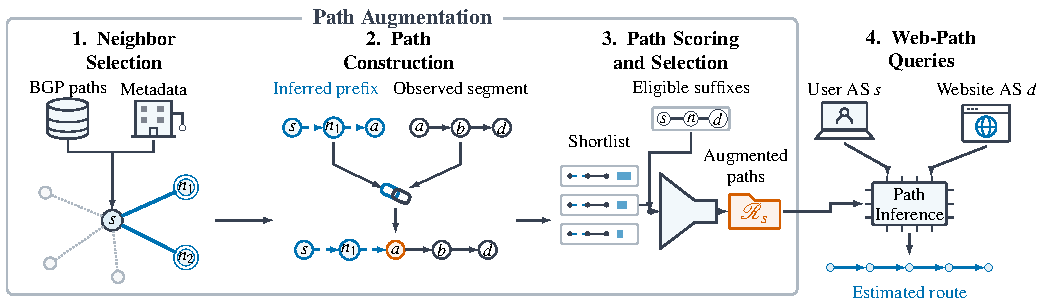
\includegraphics[width=\textwidth]{figures/fig2_overview.pdf}
\caption{\sys groups the first three steps as path augmentation, producing
a library for model training and Web-path queries. Dashed prefixes join
solid observed segments; observed suffixes enter the shared scoring and
selection stage.}
\Description{The first three scenes are enclosed in a frame labeled Path
Augmentation: neighbor selection, path construction by joining a prefix to
an observed segment, and path scoring and selection into a shared library.
The fourth scene, outside the frame, answers user-to-website path queries.}
\label{fig:overview}
\end{figure*}

\sys estimates the routes behind Web access using a source-specific path
library $\mathcal R_s$ constructed from other networks' observations and
public interconnection information. For each source and snapshot, learned
neighbor ranking and recursive exploration identify usable branches.
Stitching reuses observed segments; complete-path scoring and selection
admit candidates into the library.

Figure~\ref{fig:overview} separates path augmentation (Steps~1--3) from website queries. Shared
AS, transition, and path representations support the construction decisions.
The selected library supplies training paths and local evidence for
candidate generation, and is reused across website endpoints.

\subsection{Representing Public Routing Evidence}
\label{sec:evidence_representation}

We encode AS relationships, graph structure, network attributes,
PeeringDB co-location, and observed paths as tabular features at three
levels (Table~\ref{tab:method_features})~\cite{CAIDA,caidaASrank,PeeringDB}.
Provenance and missing or conflicting evidence remain explicit.
Co-location supplies candidate information without establishing adjacency.

\begin{table}[t]
\centering
\caption{Public evidence at AS, transition, and path levels, complemented
by destination context and uncertainty indicators.}
\label{tab:method_features}
\small
\begin{tabularx}{\columnwidth}{@{}lX@{}}
\toprule
Level & Representation and use\\
\midrule
AS and AS pair & Network size and transit role; graph connectivity and
overlap; shared PeeringDB locations. Used to rank possible neighbors.\\
Transition & Preceding, current, and next AS; directed commercial roles,
local support, and prefix-phase compatibility. Used for exploration and
prefix assessment.\\
Complete path & Ordered edge and segment support, prefix reliability,
actual third AS, and continuation evidence. Used to score constructed
routes.\\
Destination context & Donor agreement toward the same destination, with
incoming-role conditioning and equal donor-source weighting; evaluated
at the first hop and stitching boundary.\\
Uncertainty & Missing metadata, unknown or conflicting roles, absent
donor coverage, and the end of a construction boundary.\\
\bottomrule
\end{tabularx}
\end{table}


\paragraph{Destination-conditioned routing support.}
An observed route at a neighbor need not be available to the source:
learning, selecting, and exporting a BGP route are distinct
operations~\cite{rfc4271}. For a candidate $(s,n,a,\ldots,d)$, we therefore
measure whether other source networks observe $n$ followed by $a$ toward
the same destination $d$. Let $c_v(n,a,d)$ count distinct observed paths
beginning $(v,n,a)$ and ending at $d$, and let
$c_v(n,d)=\sum_b c_v(n,b,d)$. With
$V_{n,d}=\{v:c_v(n,d)>0\}$, we compute
\begin{equation}
\begin{split}
f(n,a,d)&=\frac{|\{v\in V_{n,d}:c_v(n,a,d)>0\}|}{|V_{n,d}|},\\
m(n,a,d)&=\frac{1}{|V_{n,d}|}\sum_{v\in V_{n,d}}
                    \frac{c_v(n,a,d)}{c_v(n,d)}.
\end{split}
\label{eq:destination_evidence}
\end{equation}
Here $f$ measures agreement across donor sources, while $m$ also accounts
for each donor's alternative next hops. Per-donor normalization and equal
donor weighting limit the influence of prolific observers. We also compute
these statistics using donors whose incoming commercial relationship to
$n$ matches that of the candidate's preceding AS. Only original first-hop
contexts $(v,n,a,\ldots,d)$ contribute; arbitrary internal occurrences of
$n$ do not establish this export context.

At the first hop and prefix--segment boundary, two 16-feature context
vectors and one boundary indicator add 33 features to 181 route,
32 prefix-reliability, and 9 actual-next-hop features: 255 in total.
Absent donor coverage, unknown roles, and conflicts have explicit indicators.

\subsection{Neighbor Ranking and Recursive Exploration}
\label{sec:neighbor_selection}
\label{sec:recursion}

\paragraph{Learning likely forwarding neighbors.}
For $s$, we retrieve candidate neighbors from the public AS graph,
remaining BGP observations, and PeeringDB co-location, prioritizing
graph-supported candidates within a pool of at most 4,096 ASes. We train
LightGBM~\cite{ke2017lightgbm} ranking and presence models using public and
structurally extended views. The latter adds degree-normalized overlap and
population-weighted co-location features. Training labels give each destination
equal weight, divided across its distinct observed routes. Neighbors are
ordered by this first-hop support: Top-3 neighbors receive relevance 3,
ranks 4--10 receive 2, other observed neighbors receive 1, and unobserved
neighbors receive 0. Presence labels indicate observed first-hop use.

Let $r_s^{\mathrm{str}}(n)$ be the structural ranking score and
$p_s^{\mathrm{pub}}(n),p_s^{\mathrm{str}}(n)$ the two presence scores. We use
\begin{equation}
\begin{split}
\bar p_s(n)&=\tfrac12\bigl(p_s^{\mathrm{pub}}(n)+p_s^{\mathrm{str}}(n)\bigr),\\
u_s(n)&=z\bigl(r_s^{\mathrm{str}}(n)\bigr)
          +0.5\log\frac{\bar p_s(n)}{1-\bar p_s(n)},
\end{split}
\label{eq:neighbor_ranking}
\end{equation}
where $z$ standardizes scores within the candidate pool and probabilities
are clipped before taking the logit. The union of both rankers' Top-3
candidates forms a protected core. We place it first, ordering within the
core and the remaining pool by $u_s$, then select the longest prefix
containing the core with at most 32 neighbors and mean $\bar p_s\geq0.7$.
If no such prefix exists, we retain the core and mark its support uncertain.
The output is $\mathcal N_s$; individual selected neighbors need not exceed
0.7.

A separate grouped-softmax head learns destination-balanced first-hop
importance from paths containing at least three ASes. For sample
allocation, we normalize its predicted masses over selected neighbors to
obtain $\pi_s(n)$. These are allocation weights derived from observed route
support, rather than estimates of traffic volume.

\paragraph{Exploring branches with insufficient observations.}
For a prefix $q=(s,n,\ldots,z)$, let $c(q)$ count distinct observed forward
tails that yield structurally admissible paths when joined to $q$.
Counting stops once $\tau$ usable tails are found. We retain every prefix
with $c(q)>0$ for construction. When $c(q)<\tau$, a local next-hop ranker
conditioned on the preceding AS and commercial roles identifies supported
extensions. An added edge requires observed or public connection evidence,
or co-location accompanied by a finite learned support score. Extensions
exclude repeated ASes and conflicts with the prefix's possible commercial
phases.

We use $\tau=300$, at most ten next hops per extension, and a maximum prefix
of three ASes, yielding $(s,n)$ and $(s,n,a)$ prefixes. Recursion supplements
usable direct prefixes; its trigger is observation availability, not source
degree. Expansion can expose upstream choices for sources with few exits.
A branch stops
at the prefix limit or when no supported continuation is available.

\subsection{Path Construction and Selection}
\label{sec:generation}
\label{sec:path_selection}

\paragraph{Reusing observed routing choices.}
Observed BGP segments already encode ordered routes through multiple
networks. We preserve this information by joining a selected prefix
$q=(s,\ldots,z)$ to an intact forward segment $T_{z,j}(P)$ from
Equation~\eqref{eq:collected_tail}, including $z$ once. The result must have
3--20 distinct valid ASes, admissible prefix edges, and a feasible
valley-free completion of known relationships~\cite{gao2001inferring}.
Unknown relationships remain unknown. These checks establish compatibility;
the source's use of the constructed route still requires assessment.

To bound construction while retaining alternatives, we keep up to two
evidence-prioritized candidates per first hop, actual third AS, destination,
and AS count. Priority favors fewer inferred prefix extensions and support
from more observation sources. A deterministic work budget covers 5,000
destination contexts, supplemented by protected contexts for sparse
prefixes. These construction representatives are scored as complete routes.

\paragraph{Learning complete-path observation support.}
A LightGBM classifier $h_\theta(\phi(P))$ scores the 255-feature candidate
representation, using 300 trees, at most 31 leaves per tree, depth seven,
and learning rate 0.04. For a training source, a candidate is positive if its
complete ordered sequence appears in that source's reference. A
nonmatching sequence is negative only when its destination has reference
coverage; uncovered destinations remain unknown and are excluded.
Weighted binary cross-entropy balances sources, first hops, destinations
within each first hop, and alternative paths per destination.

The scorer uses 160 training sources and 40 disjoint validation sources.
Upstream predictions for a training source come from models fitted without
its source fold; donor statistics exclude the same original-source fold
even when recursion changes the stitching AS. This is stagewise source
isolation, not fully nested end-to-end cross-fitting. Validation and target
queries use the training models and donors. Final target reference paths
do not determine features, selection, or checkpoints. Scores estimate
finite-corpus observation support, not route-existence probabilities.

\paragraph{Preserving important forwarding branches.}
High scores alone can concentrate the library on a well-observed neighbor.
We therefore combine support-based ranking with minimum sample requests
for important neighbors. A neighbor is major if it is in the Top-3 of
$\pi_s$ or has $\pi_s(n)\geq0.1$. For a nominal budget $B$ clipped to candidate
capacity, we request
\begin{equation}
L_s(n)=
\begin{cases}
\max\{50,\lceil0.5\pi_s(n)B\rceil\},&n\text{ is major},\\
1,&\text{otherwise}.
\end{cases}
\label{eq:branch_floor}
\end{equation}
Requests are clipped to available paths and shortages are recorded. The
budget can expand to retain the available mandatory paths. This preserves
samples through important neighbors without requiring equal branch counts.

After these requests, selection greedily fills the remaining budget using
the marginal gain of
\begin{equation}
F(\mathcal R)=
\sum_{P\in\mathcal R}\log\max\{h_\theta(\phi(P)),\epsilon\}
-\lambda\sum_d c_d(\mathcal R)\log c_d(\mathcal R),
\label{eq:library_selection}
\end{equation}
where $c_d$ counts selected paths to $d$, $0\log0=0$, $\epsilon=10^{-12}$,
and $\lambda=0.1$. The weak repetition penalty discourages redundant
destination sampling; selection uses a greedy approximation.

\paragraph{Integrating augmented and observed paths.}
Algorithm~\ref{alg:path_synthesis} applies this selection in two passes.
First, generated candidates form an augmentation shortlist $\mathcal U_s$,
with nominal size 1,000 and a goal of 1,000 paths absent from both the public
path index and $\mathcal K_s^{\mathrm{tr}}$, the subset of full suffixes
provided by training sources. We retain the highest-scoring overall and
previously unavailable candidate per first-hop--destination--AS-count
group. Branch and novelty requirements can expand the budget; insufficient
candidate capacity is recorded. If $|\mathcal U_s|<1{,}000$, we return it as
$\mathcal R_s$ without a fusion pass.

Otherwise, we integrate eligible full suffixes from $\mathcal K_s$.
Each preserves its observed direction and original terminal AS; its first
hop must belong to $\mathcal N_s$ and occur in $\mathcal U_s$. The pool is
\begin{equation}
\mathcal V_s=\mathcal U_s\cup\mathcal K_s^{\mathrm{eligible}}.
\label{eq:common_pool}
\end{equation}
We deduplicate ordered sequences, mark external suffixes and their overlaps
as previously available, and score the pool with the same model and
representative rule. A second selection uses budget $|\mathcal U_s|$ and the
same branch safeguards, without another novelty minimum. Thus alternatives
to the same destination compete on support and branch needs. The final
library $\mathcal R_s$ retains provenance for every selected path.

\begin{algorithm}[t]
\caption{Evidence-guided Path Augmentation}
\label{alg:path_synthesis}
\footnotesize
\begin{algorithmic}[1]
\Require Source $s$, selected neighbors $\mathcal N_s$, importance $\pi_s$
\Require Observed segments $\mathcal T$, suffixes $\mathcal K_s,\mathcal K_s^{\mathrm{tr}}$
\Require Next-hop predictor $g$, support scorer $h_\theta$
\Require $\tau=300$, $D=3$, $k=10$, $B_0=\nu_0=1{,}000$
\Ensure Selected source-specific library $\mathcal R_s$
\State $\mathcal B\gets\emptyset$; $W\gets[(s,n):n\in\mathcal N_s]$
\While{$W\ne\emptyset$}
  \State $q\gets\Call{Pop}{W}$
  \State $c\gets\Call{UsableTailCount}{q,\mathcal T,\tau}$
  \State $E\gets\{q\oplus T:T\in\mathcal T_{\mathrm{last}(q)},\ \Call{Valid}{q,T}\}$
  \State $\mathcal B\gets\mathcal B\cup E$
  \If{$c<\tau$ and $|q|<D$}
    \State $A\gets\Call{SupportedTopK}{g(s,q),k}$
    \ForAll{$a\in A$ with $a\notin q$}
      \State \Call{Push}{$W,q\mathbin{\|}(a)$}
    \EndFor
  \EndIf
\EndWhile
\State $\mathcal B\gets\Call{ConstructionReps}{\mathcal B}$
\State $\mathcal B\gets\Call{WorkBudget}{\mathcal B,5000}$
\State \Call{MarkUnavailable}{$\mathcal B,\mathcal T,\mathcal K_s^{\mathrm{tr}}$}
\State $\mathcal B\gets\Call{ScoreAndRepresent}{\mathcal B,h_\theta}$
\State $\mathcal U_s\gets\Call{Select}{\mathcal B,\pi_s,B_0,\nu_0}$
\If{$|\mathcal U_s|<B_0$}
  \State \Return $\mathcal U_s$ \Comment{record capacity shortfall}
\EndIf
\State $\mathcal K'\gets\{P\in\mathcal K_s:\Call{ValidFull}{P},$
\Statex \hspace{\algorithmicindent}$\qquad \Call{FirstHop}{P}\in\mathcal N_s\cap\Call{FirstHops}{\mathcal U_s}\}$
\State $\mathcal V\gets\Call{Deduplicate}{\mathcal U_s\cup\mathcal K'}$
\State \Call{MarkKnown}{$\mathcal V,\mathcal K'$}
\State $\mathcal V\gets\Call{ScoreAndRepresent}{\mathcal V,h_\theta}$
\State $\mathcal R_s\gets\Call{Select}{\mathcal V,\pi_s,|\mathcal U_s|,0}$
\State \Return $\mathcal R_s$ for both training and candidate generation
\end{algorithmic}
\end{algorithm}


In Algorithm~\ref{alg:path_synthesis}, $q\oplus T$ joins a prefix and
segment at their common AS, and $q\mathbin{\|}(a)$ appends a successor.
\textsc{Select}$(X,\pi,B,\nu)$ applies the branch requests and greedy
objective, with nominal budget $B$ and minimum $\nu$ previously unavailable
paths when capacity permits.

\subsection{Web-Path Inference}
\label{sec:web_queries}

Our implementation uses GMPI~\cite{li2023realizing} for the score in
Equation~\eqref{eq:downstream_inference}. Its training and local candidate
generation consume the same selected library $\mathcal R_s$. Remaining
public observations support topology-based candidate generation and
history retrieval. GMPI keeps candidate and historical paths as separate
inputs and ranks
query candidates; the support scorer governs library admission. Queries
return one estimated route, or no estimate if usable candidates are
absent. Same-AS and direct-edge cases undergo the same reference-based
evaluation.


\section{Evaluation}
\label{sec:evaluation}

\subsection{Research Questions}

We evaluate the tool in two complementary settings: a BGP experiment that
withholds source-originated paths, and traceroute measurements toward
domain-derived endpoints. The BGP setting represents destination ASes as
potential Web-service networks. The domain-endpoint setting provides
data-plane observations toward actual resolved destinations.

The evaluation asks three questions:
\textbf{RQ1}, how accurately does the tool estimate routes from a user network
to a serving network; \textbf{RQ2}, do selected first hops and anchors cover
the observed routing choices; and \textbf{RQ3}, do constructed paths represent
the selected neighbors and have complete-path observation support?

\subsection{Data and Source Withholding}

Table~\ref{tab:data_sources} lists data sources, dates, scales, and roles.

\begin{table*}[t]
\centering
\caption{Data sources, snapshot dates (2026, month--day), and uses.}
\label{tab:data_sources}
\footnotesize
\setlength{\tabcolsep}{4pt}
\renewcommand{\arraystretch}{1.0}
\begin{tabularx}{\textwidth}{@{}p{3.0cm}p{2.65cm}X@{}}
\toprule
Data source & Snapshot / period & Contents, scale, and use\\
\midrule
Route Views / RIPE RIS~\cite{RouteViews,RIPERIS}
& 02-01, 03-01, 04-01; 10-15
& Public RIB paths supply the graph, segments, and training evidence.
Ten withheld sources per month yield 685,820 / 685,765 / 688,302 test pairs;
October BGP supplies evidence for Web queries.\\
CAIDA AS Relationships~\cite{caidaASRelationships}
& 02-01, 03-01, 04-01; 10-01
& Provider--customer and peer labels for neighbor features and
routing-policy compatibility checks; missing relationships remain unknown.\\
CAIDA ASRank~\cite{caidaASrank}
& 02-01, 03-01, 04-01; 10-01
& AS and link attributes, including rank, degree, and customer-cone size,
for neighbor selection and path scoring.\\
PeeringDB~\cite{PeeringDB}
& 02-01, 03-01, 04-01; 10-14
& Network attributes and IXP / facility memberships for candidate retrieval
and interconnection features; shared presence does not establish adjacency.\\
\addlinespace
Tranco N26XW~\cite{lepochat2019tranco}
& 10-14
& Frozen list of 1,000,000 ranked domains for selecting Web measurement targets.\\
DNS resolution (this study)
& 10-15
& 911,257 resolved domains yield 388,491 unique IPv4 probe targets and
domain-to-endpoint associations.\\
CAIDA prefix-to-AS~\cite{caidaRouteviewsPfx2AS}
& 10-13, 10:00 UTC
& 1,126,405 IPv4 prefix-to-origin entries for longest-prefix mapping of
endpoints and hops; ambiguous origins remain ambiguous.\\
\addlinespace
Traceroute (this study)
& 10-15--10-16
& AS63835: 388,491 TCP + 243,207 ICMP-Paris records. Under the same-AS
gap-removal rule, 22,844 eligible records yield 2,198 distinct ordered
reference paths over 1,890 AS pairs, used only for evaluation.\\
\bottomrule
\end{tabularx}
\end{table*}


\paragraph{Controlled BGP setting.}
We use three monthly Route Views and RIPE RIS RIB
snapshots: February 1, March 1, and April 1, 2026, at 08:00 UTC.
For each date, ten sources were selected by the largest original per-source
path files. All distinct source--destination pairs form the fixed query sets.
The March snapshot included 52 Route Views and 23 RIS collectors. After
removing prefixes and duplicate AS sequences, its construction graph
contained 74,781 ASes and 537,872 edges. Its sources were 16552, 19529,
32590, 34927, 42473, 49544, 58057, 199524, 328840, and 398465.

Before constructing the graph or source-specific evidence, paths starting
at these sources were withheld. Other sources' paths could still contain
them internally and provide forward suffixes.

\paragraph{Domain-endpoint setting.}
We resolved the frozen Tranco list to IPv4 targets on October 15 and probed
from AS63835 through October 16. We retained the earliest TCP observation
per destination and used ICMP Paris traceroute for targets not reached by
TCP. The 631,698 records are measurements, not independent AS-pair queries.

We mapped hop addresses using the dated CAIDA prefix-to-AS snapshot and
collapsed consecutive copies of an ASN. Under the same-AS gap assumption,
an unknown run bounded by that ASN was removed; gaps between different ASes or at
an endpoint were not filled. Eligibility required reaching the target, a
single destination-origin mapping, matching endpoints, no remaining unknown
hop, and no AS loop. The resulting 1,890 AS pairs include one same-AS pair.
No raw record had a fully mapped continuous TTL sequence without this
assumption. The endpoints were domain-derived, not individually verified
HTTP services.

All available October 15 BGP evidence was used; AS63835 had no originating
path in that corpus. Traceroute paths were excluded from graph construction,
augmentation inputs, training, and checkpoint selection. They supplied the
reference observations for scoring the fixed queries.

\subsection{Implementation Settings}
\label{sec:implementation}

We used the GMPI ranker with 256-dimensional AS representations and a hidden
size of 512. The BGP benchmark includes KnownPath~\cite{qiu2005path} and
PathRadar~\cite{11044440} as reference methods.
For the domain-endpoint experiment, we used batch size 64,
Adam learning rate 0.001, and a maximum of 30 training epochs. A stable 10\%
split of construction-derived training pairs provided internal validation,
with early stopping after three non-improving epochs. This experiment used
random seed 20261015. Reference paths were excluded from model training and checkpoint
selection. For the domain-endpoint queries, we compared with
KnownPath~\cite{qiu2005path}, which extends known AS paths under routing
constraints. Both methods were scored on the same query pairs.

The final Jaccard scores were calculated from returned path sequences
against the reference observations, including queries handled by same-AS
and direct-edge rules.

\subsection{Metrics at Each Stage}
\label{sec:metrics}

\paragraph{Final query agreement.}
We retain AS-set Jaccard as the primary end-to-end metric. Let $S(P)$ be the
set of ASes in route $P$, including endpoints, and let $\mathcal T(q)$ contain
the distinct reference paths for fixed query $q$:
\begin{equation}
\begin{split}
J(P,T)&=\frac{|S(P)\cap S(T)|}{|S(P)\cup S(T)|},\\
\mathrm{Acc}_J&=\frac{1}{|Q|}\sum_{q\in Q}
\operatorname{round}_3
\left(\max_{T\in\mathcal T(q)}J(\widehat P_q,T)\right).
\end{split}
\label{eq:jaccard}
\end{equation}
Missing or endpoint-invalid predictions contribute zero to
\eqref{eq:jaccard}. Each fixed pair has equal weight, regardless of domain
aliases or observation multiplicity. Jaccard measures AS-set agreement;
it does not establish AS order, exact routes, or routing correctness for
every prefix.

\paragraph{Neighbor and anchor selection.}
First-hop coverage $C_1$ is the fraction of reference routes whose first
neighbor is selected, averaged within each pair and then across eligible
pairs. Same-AS paths have no first hop and are excluded.
Fixed-sparse anchor coverage $C_2$ uses sources of graph degree at most ten
and reference paths with at least three ASes and a selected first hop. It
checks whether the third AS is an admitted, enabled anchor. Selected branches
with no anchor, exhausted budgets, or disabled recursion score zero. The Web
diagnostic further conditions on branches flagged to attempt recursion, and
is named trigger-conditional anchor coverage. Both average within a pair and
then over eligible pairs. Their denominators are reported separately.

\paragraph{Branch representation.}
Let $\mathcal O_s$ be the forward first-hop neighbors witnessed in the
reference paths, and $\mathcal S_s=\mathcal N_s\cap\mathcal O_s$.
For each selected-and-witnessed neighbor, we report whether
any constructed path was generated and whether at least one generated path
matched a complete ordered reference. The two coverage denominators are
$\sum_s|\mathcal S_s|$; zero-output branches remain included.
An admitted neighbor absent from the reference is marked unverified,
rather than false. Equal generated counts are not required, and neither
the observed nor generated distribution is interpreted as traffic volume.

\paragraph{Complete-path observation support.}
Let $\mathcal R_Q$ contain distinct constructed paths whose endpoint pairs
occur in $Q$. The support rate is
\begin{equation}
U=\frac{|\{P\in\mathcal R_Q:P\in\mathcal T(\operatorname{pair}(P))\}|}
{|\mathcal R_Q|}.
\label{eq:path_support}
\end{equation}
Equation~\eqref{eq:path_support} requires complete ordered equality,
not Jaccard equal to one. Paths outside $Q$ lack a reference and are reported
separately. We also recompute support after excluding constructed paths
already present as full source-rooted sequences in $\mathcal K_s$.
An unmatched path is unsupported by this finite reference, not proven
nonexistent.

\subsection{BGP Path-Visibility Results}

\paragraph{RQ1: Returned path views.}
Table~\ref{tab:bgp_results} summarizes path-estimation results across three
monthly BGP snapshots. The stage-wise assessment below examines the
685,765 query pairs in the March snapshot.

\begin{table}[t]
\centering
\caption{Path-estimation results across three monthly BGP snapshots.
KnownPath uses 10,000 sampled pairs per date; PathRadar and \sys use
the full query sets.}
\label{tab:bgp_results}
\footnotesize
\setlength{\tabcolsep}{2pt}
\begin{tabular*}{\columnwidth}{@{\extracolsep{\fill}}llrr@{}}
\toprule
Date & Method & Scored pairs & Jaccard\\
\midrule
2026-02-01 & KnownPath & 10,000 & 72.10\%\\
 & PathRadar & 685,820 & 68.73\%\\
 & \sys & 685,820 & 80.02\%\\
\midrule
2026-03-01 & KnownPath & 10,000 & 70.43\%\\
 & PathRadar & 685,765 & 68.46\%\\
 & \sys & 685,765 & 78.99\%\\
\midrule
2026-04-01 & KnownPath & 10,000 & 72.15\%\\
 & PathRadar & 688,302 & 68.44\%\\
 & \sys & 688,302 & 80.31\%\\
\midrule
Mean & KnownPath & 10,000 & 71.56\%\\
 & PathRadar & 686,629 & 68.54\%\\
 & \sys & 686,629 & 79.77\%\\
\bottomrule
\end{tabular*}
\end{table}

\paragraph{RQ2: Exit and anchor coverage.}
Selected first hops covered 84.52\% of the observed routes under pair-balanced
aggregation. On the sparse-source cohort of 137,394 eligible pairs, anchor
coverage $C_2$ was 85.10\%. These metrics assess the inferred prefix
separately from the complete route: a covered exit does not establish that
every continuation through that exit is used by the source.

\paragraph{RQ3: Branch representation and complete-path support.}
Table~\ref{tab:stage_results} reports the evidence-construction results.
Of 152 admitted source--neighbor relations, 143 were witnessed in the
reference paths. Constructed paths represented 142 of these branches
(99.30\%); 135 branches (94.41\%) had at least one constructed path matching
a complete ordered reference. The branch from AS328840 to AS328913
produced no admissible path. The method therefore retained evidence across
most selected, witnessed neighbors, without guaranteeing coverage of every
branch.

\begin{table}[t]
\centering
\caption{Selection and constructed-path assessment for the BGP setting.
Branch coverage uses the 143 selected-and-witnessed neighbors. Complete-path
support uses the 140,762 constructed paths with reference-covered AS pairs.}
\label{tab:stage_results}
\footnotesize
\setlength{\tabcolsep}{3pt}
\begin{tabularx}{\columnwidth}{@{}Xr@{}}
\toprule
Metric & \sys\\
\midrule
Admitted source--neighbor relations & 152\\
Selected, reference-witnessed neighbors & 143\\
Witnessed branches with generated paths & 142/143\\
Witnessed branches with complete-path support & 135/143\\
First-hop coverage $C_1$ & 84.52\%\\
Sparse-source anchor coverage $C_2$ & 85.10\%\\
Distinct constructed paths & 141,277\\
Reference-evaluable constructed paths & 140,762\\
Ordered supported paths & 106,326\\
Complete-path support $U$ & 75.54\%\\
Support excluding known full sequences & 74.54\%\\
Paths without a reference pair & 515\\
\bottomrule
\end{tabularx}
\end{table}

Among the 140,762 evaluable constructed paths, 106,326 matched a complete
ordered reference sequence, giving 75.54\% support. After excluding paths
already available as known full source-rooted sequences, support was
74.54\% (98,420 of 132,028 paths). This distinguishes support for assembled
routes from reuse of known complete routes. The 515 paths without a
reference pair were not assigned a support score.

\subsection{Domain-Endpoint Results}
\label{sec:web_validation}

The domain-endpoint experiment evaluated the network paths behind Web access
from AS63835. Table~\ref{tab:web_results} reports the same fixed-pair Jaccard
metric for \sys and KnownPath.

\begin{table}[t]
\centering
\caption{Path estimates toward domain-derived endpoints from AS63835.
Both methods are scored on the same 1,890 AS pairs, with missing predictions
contributing zero. Reference sequences use the same-AS gap-removal assumption.}
\label{tab:web_results}
\footnotesize
\setlength{\tabcolsep}{3pt}
\begin{tabularx}{\columnwidth}{@{}Xrr@{}}
\toprule
Method & Valid outputs & Jaccard\\
\midrule
KnownPath & 1,866 & 69.19\%\\
\sys & 1,837 & 69.96\%\\
\bottomrule
\end{tabularx}
\end{table}

\sys obtained 69.96\% Jaccard, compared with 69.19\% for KnownPath.
KnownPath returned more valid outputs, while \sys had higher mean
AS-set agreement over the full query set. This result concerns the
single measured source and the selected endpoint mappings.

The selected first hop was AS4134, with $C_1=99.09\%$ over 1,889 cross-AS
pairs. Recursive anchors AS1299, AS2914, and AS3356 gave trigger-conditional
anchor coverage of 58.37\% over 1,879 eligible pairs. This illustrates the
single-neighbor setting: knowing the first hop leaves choices about the
continuation beyond that neighbor.

The construction produced 12,849 distinct paths. Of these, 744 had a
reference-covered AS pair, and 395 matched a complete ordered reference,
giving 53.09\% support on the evaluable subset. The remaining 12,105 paths
lacked a reference pair and were not scored as either supported or false.
Consequently, 53.09\% describes the reference-covered subset, not all
constructed paths.

\section{Discussion}
\label{sec:discussion}

\paragraph{What the path view could support.}
A user could compare estimated routes to news, shopping, and video endpoints
to identify recurring transit networks or inspect networks of concern.
A content provider could issue the same queries from several user ASes
toward candidate serving ASes and examine differences in estimated network
dependencies. The tool supplies routing information for such analysis.
It does not itself steer traffic around an AS, select a deployment, or
measure the resulting performance or security benefit. AS-set agreement
also does not validate an individual AS-avoidance decision.

\paragraph{Network and measurement scope.}
The ten BGP sources were selected for their large original path files.
Withholding their paths does not make them representative of poorly observed
access networks. The Web measurement adds one measurement vantage, not
global user coverage. Endpoint mapping, prefix-specific policies, intra-AS
routing, and routing drift limit the AS-pair view. The same-AS gap assumption
can conceal an unobserved detour, and incomplete traceroute responses do not
establish a packet-perfect route.

\paragraph{Evidence and validation limits.}
Compatibility checks and learned observation-support scores cannot prove
that a constructed path is selected for a particular prefix. The BGP cohort also informed
method development; its results do not establish generalization to unseen
dates. The domain-endpoint experiment adds a complementary measurement
setting, but uses one source and one random seed. Broader source and date
coverage, repeated training, score calibration, and sensitivity to library
selection remain limitations of the present evaluation.

\section{Conclusion}
\label{sec:conclusion}

We have presented \sys, a tool for estimating the networks behind Web access
from shared public evidence. It constructs reusable source-specific paths
through learned neighbor selection, evidence-capacity expansion, and
complete-path scoring, then uses an existing ranker to answer
user-network--endpoint queries. The three-snapshot BGP benchmark obtains approximately 80\% AS-set Jaccard, and the single-source
Web experiment obtains 69.96\%.
Stage-wise evaluation distinguishes selected exits, represented branches,
and supported complete paths, exposing limitations hidden by a final
aggregate score. The resulting view supports further study of Web routing
dependencies; deployment and security benefits require direct evaluation.

\clearpage
\balance
\bibliographystyle{ACM-Reference-Format}
\bibliography{ref}
\end{document}
